\begin{frame}{Wrinkling of a confined porous layer}

\bigskip
\structure{Fluorescent yoghurt makers}

\bigskip
\begin{tabu}{X[c]X[c]c}
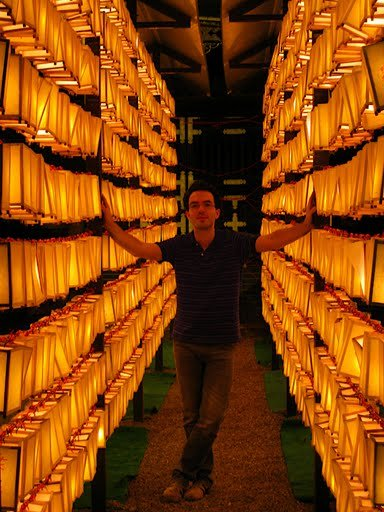
\includegraphics[height=0.3\textheight,clip=true,trim=3cm 7cm  2cm 5cm]{Mathieu}&
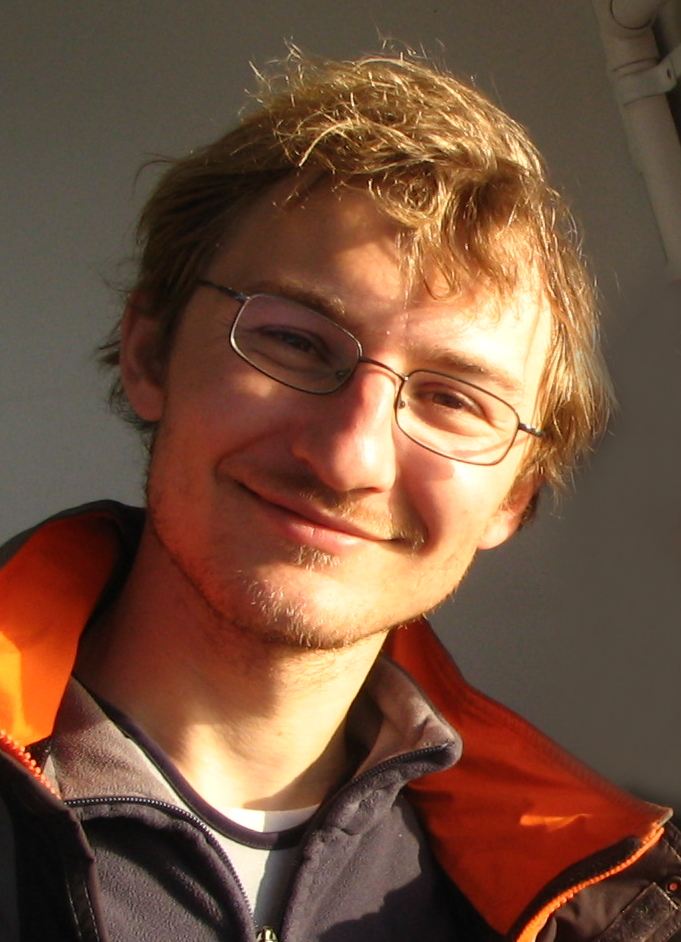
\includegraphics[height=0.3\textheight]{Thomas}&
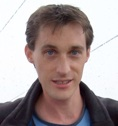
\includegraphics[height=0.3\textheight]{Seb}\\
Mathieu Nespoulous & Thomas Gibaud & Sebastien Manneville\\
Associate Professor & CNRS researcher & Professor\\
Aix-Marseille Universit\'{e} & E.N.S. Lyon & E.N.S. Lyon\\
\end{tabu}

\bigskip
\structure{Imaging plateform} BioSciences Gerland - Lyon Sud (UMS~3444)
\end{frame}


\begin{frame}{Sealed cell, spontaneous pattern}
	
	\structure{Side view of the cell}\\
	\tikzsetnextfilename{cell_brushes}
	\begin{tikzpicture}[font=\footnotesize]
		\fill[pattern=north east lines,pattern color=Accent2] (0,0) rectangle (\textwidth,1.5em) node[midway,fill=white,inner sep=1pt] {glass};
		\fill[pattern=north east lines,pattern color=Accent2] (0,-2.5em) rectangle (\textwidth,-4em) node[midway,fill=white,inner sep=1pt] {glass};
		\draw[line width=2pt,Accent1] (0.05\textwidth,-2.5em) -- (0.95\textwidth,-2.5em) (0.05\textwidth,-1pt) -- (0.95\textwidth,-1pt) node[below,pos=0.30, text width=0.5\textwidth] {acrylamide brush ($10\sim 100$ nm)\linebreak $\Rightarrow$ No adhesion};
		\fill[gray] (0,0) rectangle (0.05\textwidth,-2.5em) (\textwidth,0) rectangle (0.95\textwidth,-2.5em) node[pos=1, above left] {spacer};
		\draw[<->] (0.75\textwidth,-2pt) -- (0.75\textwidth,-2.5em) node[midway,left] {$e\sim 100\,\mu m$};
		\draw[<->] (0.05\textwidth,2.25em) -- (0.95\textwidth,2.25em) node[midway,above] (L){$L\sim 2.5\,cm$};
		%\node[anchor=north west, inner sep=0] at ($(L.north) - (0.5\textwidth,0)$) {\structure{Side view of the cell}};
	\end{tikzpicture}
	
	\bigskip
	\structure{Top view of the final pattern}\\
	\tikzsetnextfilename{patterns_zooms}
	\begin{tikzpicture}[inner sep=0, very thick]
	\setlength{\mylength}{\columnwidth}
	\node[anchor=north west] (a) {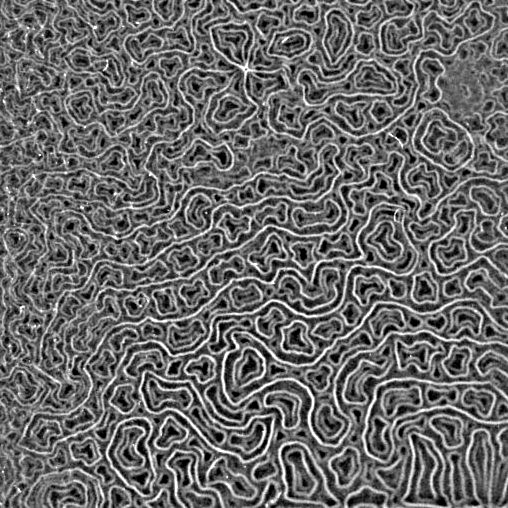
\includegraphics[width=0.28\mylength]{cas3p2_fluo0p8_GDL4_50um_coating_2_zoom2_crop}};
		\node[anchor=north] at (0.44\mylength,0) (b) {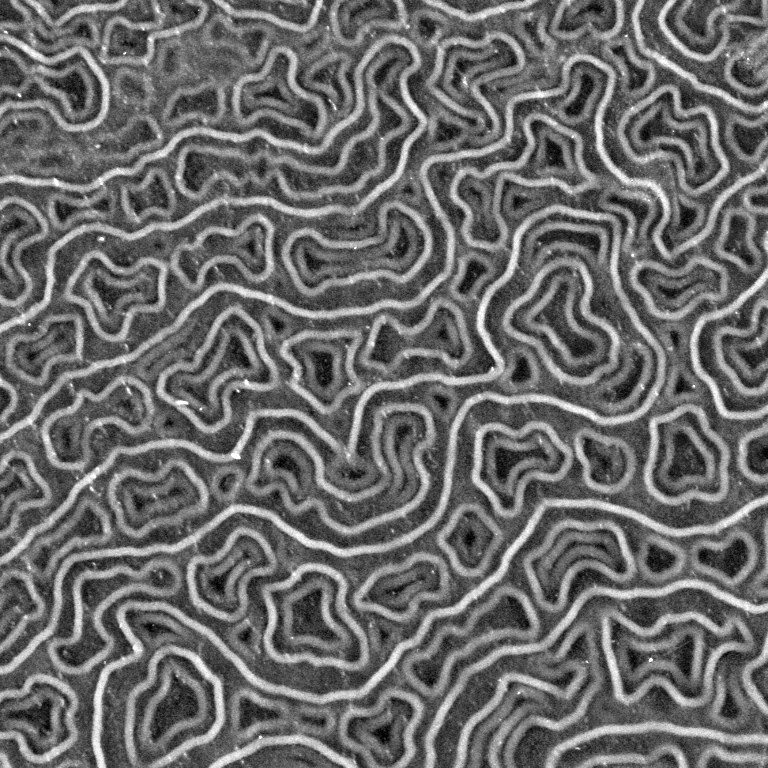
\includegraphics[width=0.28\mylength]{cas3p2_fluo0p8_GDL4_50um_coating_2_zoom6_crop}};
		\node[anchor=north east] at (\mylength,0) (c) {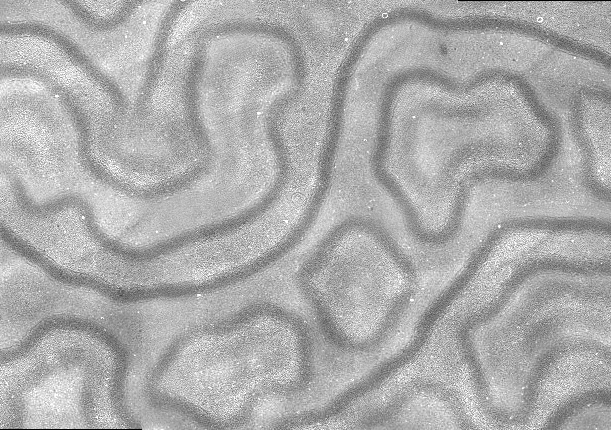
\includegraphics[width=0.4\mylength]{cas3p2_fluo0p8_GDL4_50um_coating_2_transmission}};
		%zooms
		\node[minimum width = 0.137\mylength, minimum height=0.137\mylength, anchor=north west, draw=Accent2] at ($(a.north west) +(0.111\mylength,-0.072\mylength)$) (bz){};
		\draw[Accent2] (bz.north east) -- (b.north west) (bz.south east) -- (b.south west);
		\node[minimum width = 0.128\mylength, minimum height=0.081\mylength, anchor=north west, draw=Main] at ($(b.north west) +(0.097\mylength,-0.143\mylength)$) (cz){};
		\draw[Main] (cz.north east) -- (c.north west) (cz.south east) -- (c.south west);
		\node[minimum width = 0.156\mylength, minimum height=0.156\mylength, anchor=north west, draw=Accent1] at ($(c.north west) + (0.125\mylength,0)$) (dz) {};
		%scale bars
		\draw[ultra thick] (a.south east) ++(0,-0.25em) -- ++(-0.178\mylength,0) node[pos=0.5, below=0.25em, font=\small] (M) {\SI{1}{\centi\metre}};
		\draw[ultra thick] (b.south east) ++(0,-0.25em) -- ++(-0.176\mylength,0) node[pos=0.5, below=0.25em, font=\small] {\SI{5}{\milli\metre}};
		\draw[ultra thick] (c.south east) ++(0,-0.25em) -- ++(-0.132\mylength,0) node[pos=0.5, below=0.25em, font=\small] {\SI{1}{\milli\metre}};
	\end{tikzpicture}
\end{frame}

\begin{frame}{Dynamics (transmission macroscope)}
\movie[externalviewer]{\tikzsetnextfilename{dynamics_still}\begin{tikzpicture}
\node[inner sep=0] (a) {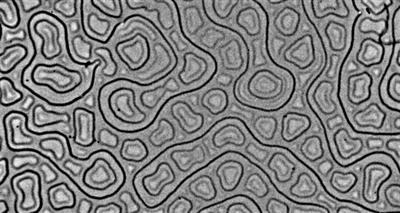
\includegraphics[width=\textwidth]{prise_0799_resized.jpg}};
\draw[line width=0.2em] ++(a.north west) -- ++(0.177\textwidth,0) node[pos=0, above right, inner xsep=0] {\SI{1}{\milli\metre}};
\end{tikzpicture}
}{cas4_GDL_4_100um_coat_macroscope_2.avi}
\end{frame}

\begin{frame}{Dynamics (transmission macroscope)}
\tikzsetnextfilename{snapshots_macroscope}
\begin{tikzpicture}
	\matrix[matrix of nodes, inner sep=0, column sep=0.015\textwidth, row sep=0.5em, ampersand replacement=\&] (m){
	33 min \& 38 min \& 43 min \\
	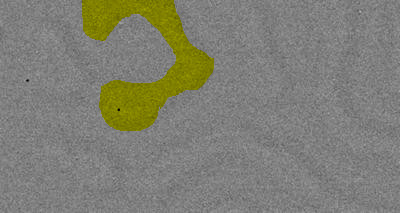
\includegraphics[width=0.32\textwidth]{prise_0100_color.jpg}\&
	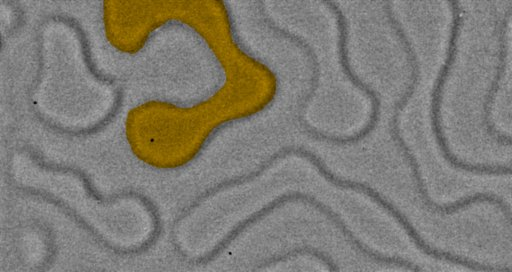
\includegraphics[width=0.32\textwidth]{prise_0130_color.jpg}\&
	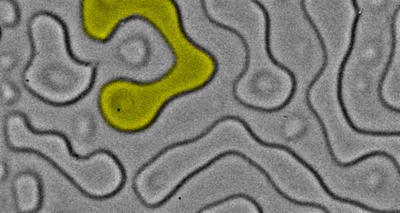
\includegraphics[width=0.32\textwidth]{prise_0160_color.jpg}\\
	48 min \& 1h \& 1h15 \\
	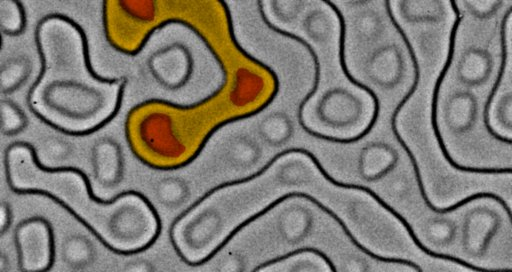
\includegraphics[width=0.32\textwidth]{prise_0190_color.jpg}\&
	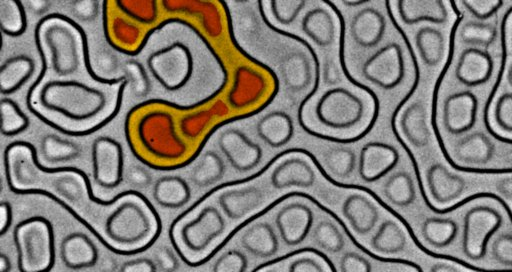
\includegraphics[width=0.32\textwidth]{prise_0250_color.jpg}\&
	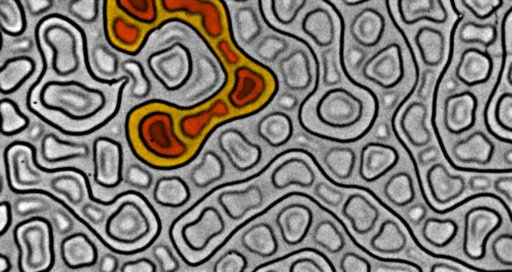
\includegraphics[width=0.32\textwidth]{prise_0360_color.jpg}\\
	};
	\draw[line width=0.2em] ++(m-4-1.south west) -- ++(0.056\textwidth,0) node[pos=0, below right, inner xsep=0] {\SI{1}{\milli\metre}};
\end{tikzpicture}

\begin{itemize}
\item nesting patterns
\item length scale becomes smaller
\end{itemize}
\end{frame}

\begin{frame}{What is going on in the thickness?}
\begin{columns}
\column{0.4\textwidth}
\begin{itemize}
\item fluorescent casein
\item confocal microscope
\item[$\Rightarrow$] 3D concentration field
\end{itemize}

\tikzsetnextfilename{scalebar_fluo}
\begin{tikzpicture}
\draw[ultra thick] (0,) -- +(0.786\textwidth,0) node[midway, above] {\SI{1}{\milli\metre}};
\end{tikzpicture}
\setlength{\tabcolsep}{1pt}
\begin{tabular}{p{\columnwidth}l}
	
\includegraphics[width=\columnwidth, height=0.061\columnwidth]{coupe_cloque_t000.png}& \SI{15}{\minute}\\
	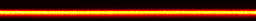
\includegraphics[width=\columnwidth, height=0.061\columnwidth]{coupe_cloque_t011.png} & \SI{22}{\minute}\\
	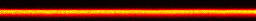
\includegraphics[width=\columnwidth, height=0.061\columnwidth]{coupe_cloque_t110.png} & \SI{1}{\hour}~26\onslide<2->{\\
	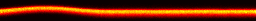
\includegraphics[width=\columnwidth, height=0.061\columnwidth]{coupe_cloque_t116.png} & \SI{1}{\hour}~30\\
	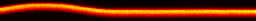
\includegraphics[width=\columnwidth, height=0.061\columnwidth]{coupe_cloque_t117.png} & \SI{1}{\hour}~31\\
	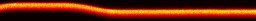
\includegraphics[width=\columnwidth, height=0.061\columnwidth]{coupe_cloque_t123.png} & \SI{1}{\hour}~35\\
	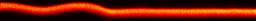
\includegraphics[width=\columnwidth, height=0.061\columnwidth]{coupe_cloque_t200.png} & \SI{2}{\hour}~25\\
	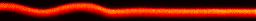
\includegraphics[width=\columnwidth, height=0.061\columnwidth]{coupe_cloque_t221.png} & \SI{2}{\hour}~40\\}
\end{tabular}

\begin{itemize}
\item synæresis and swelling
\item<2-> cause buckling
\end{itemize}
\column{0.1\textwidth}

\column{0.5\textwidth}
\tikzsetnextfilename{volume_area}
\begin{tikzpicture}
	\begin{groupplot}[%
		group style={
			group name=g, group size=1 by 3,
			xticklabels at=edge bottom,
			vertical sep=0,
			},
		xmin=0, xmax=170, xtick={0,30,...,150},
		extra tick style={grid=major},%
		extra x ticks = {21,68}, extra x tick labels={},%
		scale only axis,
		width=\textwidth-4em,
		height=5\baselineskip,
		ylabel absolute, every axis y label/.append style={anchor=base, yshift=-1em}
		]
	\nextgroupplot[
		ylabel={$G^\prime$ (\si{\pascal})},
		ymin=0,
		]
	\addplot+[no marks,Accent1] table[x expr={\thisrowno{0}/60}]{cas4_GDL4_Y271.prise};
	\node[below left] at (rel axis cs:1,1) {rheometer (stick)};
	
	\nextgroupplot[
		ylabel={Volume (\%)}, ymin=20, ymax=100, 
		ytick={40,60,80,100}, every axis y label/.append style={xshift=0.5em},
		]
	\addplot+[no marks,Accent1] table[x expr={\thisrowno{0}+15}, y expr={\thisrowno{1}*100}]{relative_volume_excess_area_cloques.txt};
	%\addplot+[only marks,Accent2, mark=+] table[y expr={\thisrowno{1}*100}]{volume_rel_half_cas8_toi.txt};
	\node[anchor=south west] at (rel axis cs:0,0) {\rotatebox{90}{synæresis}};
	\node at (axis cs:68,80) {swelling};
	
	\nextgroupplot[
		ylabel={Excess area (\%)}, ymin=0, ymax=4, ytick={0,1,2,3},
		xlabel={time (min)}, 
		every axis y label/.append style={xshift=-1em},
		]
	\only<2->{\addplot+[no marks,Accent1] table[x expr={\thisrowno{0}+15}, y expr={\thisrowno{2}*100}]{relative_volume_excess_area_cloques.txt} node[pos=1, below left] {all};
	\addplot+[no marks,Accent2] table[x expr={\thisrowno{0}+15}, y expr={\thisrowno{3}*100}]{relative_volume_excess_area_cloques.txt} node[pos=1, left] {single blister};
	\draw[->] (axis cs: 21, 3) -- (axis cs: 68, 3) node[midway, below] {\SI{1}{\hour}};}
	%\legend{all, single blister};
	\end{groupplot}
	\end{tikzpicture}
\end{columns}
\end{frame}

\begin{frame}{Dynamics (confocal microscope)}
\tikzsetnextfilename{dynamics_confocal_still}
\movie[externalviewer]{\begin{tikzpicture}
	\node[inner sep=0] (a) {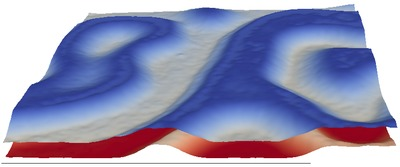
\includegraphics[width=\textwidth]{cas3p2_fluo0p8_GDL4_2_t260_crop_resized.jpg}};
	\draw[line width=0.2em] ++(a.south west) -- ++(0.75\textwidth,0) node[pos=0, below right, inner xsep=0] {\SI{1}{\milli\metre}};
	
	\node[above=1em of a, inner sep=0] (c) {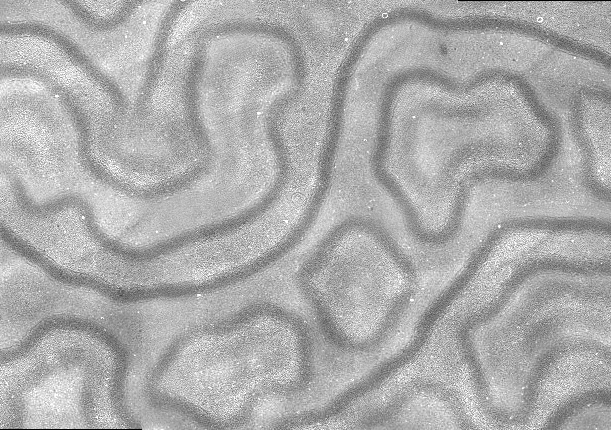
\includegraphics[width=0.4\textwidth]{cas3p2_fluo0p8_GDL4_50um_coating_2_transmission}};

	\node[minimum width = 0.156\textwidth, minimum height=0.156\textwidth, anchor=north west, draw=Accent1] at ($(c.north west) + (0.125\textwidth,0)$) (dz) {};
	\draw[ultra thick] (c.south east) ++(0,-0.25em) -- ++(-0.132\textwidth,0) node[pos=0.5, below=0.25em, font=\small] {\SI{1}{\milli\metre}};
\end{tikzpicture}
}{volume_plis_comp.avi}
\end{frame}

\begin{frame}{Dynamics (confocal microscope)}
\tikzsetnextfilename{snapshots_confocal}
\begin{tikzpicture}
	\matrix[matrix of nodes, inner sep=0, column sep=0.015\textwidth, row sep=0.5em, ampersand replacement=\&] (m){
	33 min \& 38 min \& 43 min \\
	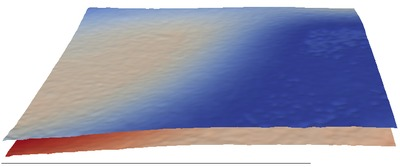
\includegraphics[width=0.32\textwidth]{cas3p2_fluo0p8_GDL4_2_t047_crop_resized.jpg}\&
	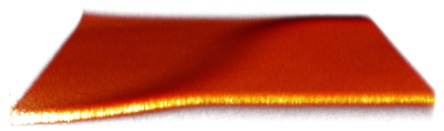
\includegraphics[width=0.32\textwidth]{cas3p2_fluo0p8_GDL4_2_t056_crop_resized.jpg}\&
	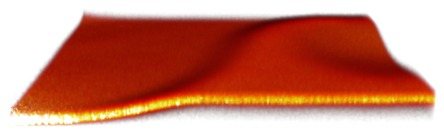
\includegraphics[width=0.32\textwidth]{cas3p2_fluo0p8_GDL4_2_t065_crop_resized.jpg}\\
	48 min \& 1h \& 1h15 \\
	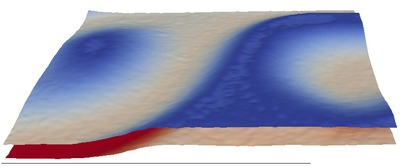
\includegraphics[width=0.32\textwidth]{cas3p2_fluo0p8_GDL4_2_t074_crop_resized.jpg}\&
	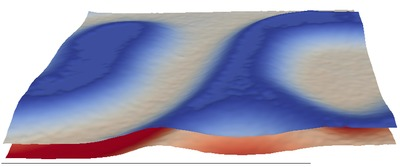
\includegraphics[width=0.32\textwidth]{cas3p2_fluo0p8_GDL4_2_t092_crop_resized.jpg}\&
	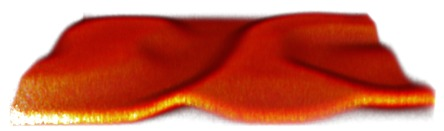
\includegraphics[width=0.32\textwidth]{cas3p2_fluo0p8_GDL4_2_t125_crop_resized.jpg}\\
	};
	\draw[line width=0.2em] ++(m-4-1.south west) -- ++(0.24\textwidth,0) node[pos=0, below right, inner xsep=0] {\SI{1}{\milli\metre}};
\end{tikzpicture}

\begin{columns}
\column{0.32\textwidth}
\begin{itemize}
\item confinement
\item cascade buckling
\item wavelength division
\end{itemize}
\column{0.68\textwidth}
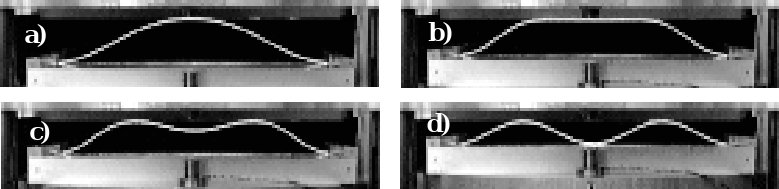
\includegraphics[width=\columnwidth]{Roman_1999_confined.jpg}

\textit{\footnotesize Roman \& Pocheau, EPL (1999)}
\end{columns}

\begin{center}
\alert{Where does the initial wavelength come from?}
\end{center}
\end{frame}


\begin{frame}<1-2>[label=carpet]{Wavelength: resisting stress needed}
\structure{Simple case} Initial flat contact with the substrate: carpet
\begin{columns}
\column{0.5\textwidth}
\temporal<2>{
	
\includegraphics[width=\columnwidth, height=0.061\columnwidth]{coupe_cloque_t000.png}\\
	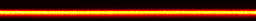
\includegraphics[width=\columnwidth, height=0.061\columnwidth]{coupe_cloque_t011.png}\\
	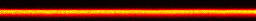
\includegraphics[width=\columnwidth, height=0.061\columnwidth]{coupe_cloque_t110.png}\\
	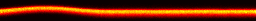
\includegraphics[width=\columnwidth, height=0.061\columnwidth]{coupe_cloque_t116.png}\\
	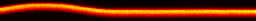
\includegraphics[width=\columnwidth, height=0.061\columnwidth]{coupe_cloque_t117.png}\\

	\movie[externalviewer]{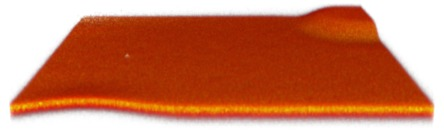
\includegraphics[width=\textwidth]{volume_cloque_t116}}{volume_cloques_comp.avi}\\
	\only<1>{\tikzsetnextfilename{cloques_still}
	\begin{tikzpicture}
	\draw[ultra thick] (0,) -- +(0.786\textwidth,0) node[midway, below] {\SI{1}{\milli\metre}};
	\end{tikzpicture}}
	
	\structure{In our case}
	\begin{itemize}
	\item Vertical cells show the same wavelength
	\item $\sigma \neq \rho g h$
	\end{itemize}
}{

\bigskip
\begin{itemize}
\item solvent must flow through gel
\begin{description}[$\ell_p$]
\item[$v$] gel velocity = -volumic flux $\simeq \SI{0.2}{\micro\metre\per\second}$
\item[$\alpha$] permeability $ \approx \SI{6e-14}{\square\metre}$
\end{description}
\item $\sigma$ is a Darcy pressure
\[\sigma = \Delta P \sim \eta h v/\alpha\]
\item poroelastic length
\[ \lambda^* \sim \left(\frac{B \alpha}{\eta v h}\right)^\frac{1}{3} \simeq \SI{0.5}{\milli\metre}\]
\end{itemize}
}{
\tikzsetnextfilename{alts_bottom_cloque}
\begin{tikzpicture}
\begin{axis}[
	width=\textwidth,
	height=0.6\textwidth,
	xmin=0, xmax=1000, xtick={0,250, 500, 750}, xlabel={position (\si{\micro\metre})},
	ymin=0, ymax=50, ylabel={altitude (\si{\micro\metre})},
	cycle list name=earthy,
	no marks,
	]
	\draw[ultra thick, Accent2] (axis cs:580,0) -- (axis cs:580,50);
	\foreach \x in {2,3,..., 8}
		\addplot table[y index=\x]{alts_bottom_cloque.txt};
\end{axis}
\end{tikzpicture}
\begin{itemize}
\item $\lambda$ frozen at ceiling touch 
\item Amplitude $A=e-h$
\item $\epsilon = \left(\frac{e-h}{\lambda^*}\right)^\frac{7}{4}$
\item $\lambda \sim \left(e-h\right)^\frac{1}{4} \left(\lambda^*\right)^\frac{3}{4}$
	%\[ \epsilon \sim \left(\frac{\lambda}{e}\frac{e}{H}\right)^{-7/3} \simeq 0.6\% \]
\end{itemize}
}

\column{0.5\textwidth}
\begin{block}{Ruck in a rug}
\tikzsetnextfilename{ruck}%
\begin{tikzpicture}[ultra thick]
\begin{axis}[
	name=a,
	width=\textwidth, height=3\baselineskip, scale only axis,
	domain=-180:180, no markers, ymin=0, ymax=3,xmin=-180,xmax=180,
	axis lines=none, xtick=\empty,
	axis background/.style={fill=white},
	]
	\addplot+[Accent1]{cos(x)+1};
	\addplot+[Accent1]{cos(x)+1.5};
	\draw[->, Accent2, ultra thick] (axis cs:90,1.25) -- (axis cs:90,2.25) node[pos=1, right] {$v$};
	\draw[Main, ultra thick,->] (axis cs:-90,1.5) -- (axis cs:-90,0.25) node[right] {$\sigma$};
	%\node[above] at (axis cs:-90,1.5) {$P_2$};
	%\node[below right] at (axis cs:-90,1.25) {$P_1$};
	\draw[<->, ultra thick] (axis cs:0,0) -- (axis cs:0,2) node[midway, right] {$A$};
	\draw[<->] (axis cs:0,2) -- (axis cs:0,2.5) node[midway, right] {$h$};
\end{axis}
\fill[pattern=north east lines,pattern color=Accent2] (a.south west) rectangle ($(a.south east)+(0,-1em)$);
\draw[<->] ($(a.south west)+(0,-1.1em)$) -- ($(a.south east)+(0,-1.1em)$) node[midway, below] {$\lambda$};
\end{tikzpicture}

\textit{\footnotesize Kolinski et al., Vella et al. PRL 2009}\\
\begin{description}[$B$]
\item[$\epsilon$] excess area \hfill$\Rightarrow$ buckling 
\item[$B$] bending modulus \hfill$\Rightarrow \lambda\nearrow$
\item[$\sigma$] vertical stress \hfill$\Rightarrow \lambda\searrow$
\end{description}
\[ \lambda^* \equiv \left(\frac{B}{\sigma}\right)^{1/3}\text{, eg. }\sigma =\rho g h \]
$\lambda \sim \epsilon^{1/7} \lambda^*$ and $A \sim \epsilon^{4/7} \lambda^*$
\end{block}
\end{columns}
\end{frame}

\begin{frame}{Poroelasticity}
\begin{columns}\column{0.15\textwidth}
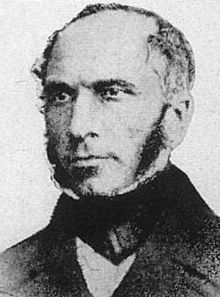
\includegraphics[width=\textwidth]{Henry_Darcy}
\column{0.85\textwidth}
\begin{block}{Henry Darcy (1803-1858)}
\begin{description}[1803]
\item[1846] granted lifelong free water
\item[1856] \textit{Les fontaines publiques de la ville de Dijon}
\end{description}
\end{block}
\end{columns}

\begin{columns}
\column{0.15\textwidth}
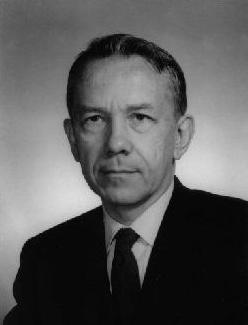
\includegraphics[width=\textwidth]{Maurice_Anthony_Biot}
\column{0.58\textwidth}
\begin{block}{Maurice Anthony Biot (1905-1985)}
\begin{description}[1803]
%\item[1932] Ph.D. under von Kármán (Cal Tech)
\item[1932-1942] earthquake engineering
\item[1935-1962] theory of poroelasticity
\end{description}
\end{block}
\column{0.27\textwidth}
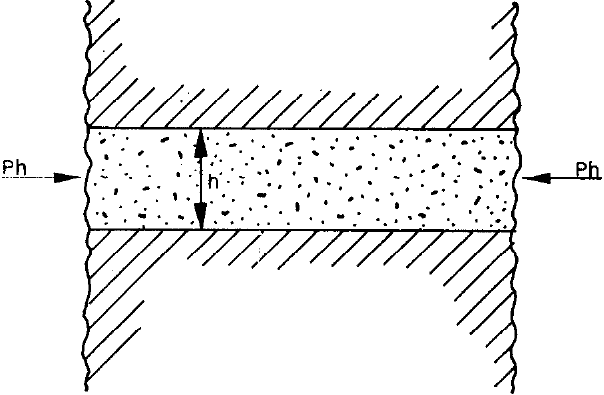
\includegraphics[width=\textwidth]{Biot_1964_Buckling_Porous}
\end{columns}

\medskip
\begin{footnotesize}
\textit{Biot, J. Appl. Mech. 1964}: Buckling of a porous slab embedded in an impervious infinite viscous or viscoelastic medium
\end{footnotesize}
\begin{itemize}
\item $B$ transiently higher due to pore pressure
\item $\sigma$ comes only from the surrounding medium $\rightarrow 0$
\item effect of flow through the porous slab not considered
\end{itemize}
\end{frame}

\begin{frame}{No initial contact with a substrate}
\structure{Poiseuille vs Darcy on a flying carpet}
\tikzsetnextfilename{flying_carpet}%
\begin{tikzpicture}
\begin{axis}[
	name=a,
	width=\textwidth, height=0.25\textwidth, scale only axis,
	domain=0:360, no markers, ymin=-4, ymax=4,xmin=0,xmax=360,
	axis lines=none, xtick=\empty,
	]
	\fill[gray!20] (axis cs:85,4) rectangle (axis cs:95,-4) (axis cs:265,4) rectangle (axis cs:275,-4);
	\addplot+[Accent1]{sin(x)+0.5};
	\addplot+[Accent1]{sin(x)-0.5};
	\addplot+[dashed, black]{0.5};
	\addplot+[dashed, black]{-0.5};
	\draw[<->, help lines] (axis cs:180,0.5) -- (axis cs:180,4) node[midway, left] {$H$}; 
	\draw[<->, help lines] (axis cs:30,-0.5) -- (axis cs:30,-4) node[midway, left] {$H$};
	\node[below] at (axis cs:90,-1.5) (pb1) {$P_1$};
	\node[above] at (axis cs:90,1.5) (ph2) {$P_2$};
	\node[above] at (axis cs:270,1.5) (ph1) {$P_1$};
	\node[below] at (axis cs:270,-1.5) (pb2) {$P_2$};
	\draw[line width=0.1em, ->] (ph2) -- (axis cs:90,0.5) node[midway, left] {Darcy} node[midway, right] {$v$};
	\draw[line width=0.1em, ->] (pb2) -- (pb1) node[midway, above] {Poiseuille} node[midway, below] {$u \sim \frac{\lambda}{H} v$};
\end{axis}
\fill[pattern=north east lines,pattern color=Accent2] (a.south west) rectangle +(\textwidth,-1em) (a.north west) rectangle +(\textwidth,1em);
\end{tikzpicture}

\begin{columns}
\column{0.17\textwidth}
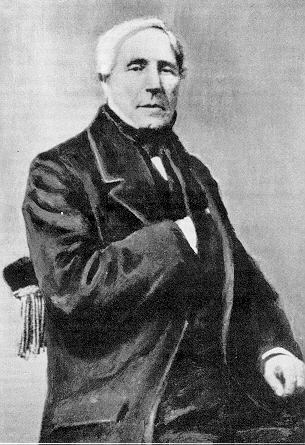
\includegraphics[width=\textwidth]{Jean-Leonard-Marie_Poiseuille.jpg}\\
\hfill\structure{1797-1869}

\column{0.80\textwidth}
The same $\Delta P$ can be relaxed by a Poiseuille flow
\begin{align*}
\Delta P &\sim 12\eta\frac{\lambda}{H^2} u \sim 12\eta\frac{\lambda^2}{H^3} v\\
\lambda^* &= \left(\frac{B H^2}{12\eta\lambda}\right)^{1/3}
\end{align*}
\textit{\footnotesize Huang \& Suo, J. Appl. Phys. (2002)}
%\item For the same wavelength
%\hfill$\displaystyle \frac{v_\text{Darcy}}{v_\text{Poiseuille}} \sim \frac{\ell_p^2\lambda^2}{hH^3} \approx 30$
%\item Flow through the pores dominates

\end{columns}
\end{frame}

\againframe<3>{carpet}

\begin{frame}{Poiseuille vs Darcy}
\begin{columns}
\column{0.5\textwidth}
\begin{block}{Observable wavelengths}
Same magnitude (typical sample)
\begin{align*}
\lambda_D &\sim \Upsilon^\frac{1}{4} h^\frac{1}{2} \alpha^\frac{1}{4}\simeq \SI{0.23}{\milli\metre}\\
\lambda_P &\sim \Upsilon^\frac{1}{6} h^\frac{1}{2} H^\frac{1}{2}\simeq \SI{0.25}{\milli\metre}
\end{align*}
\end{block}
with $\Upsilon = \frac{E(e-h)}{\eta v}\simeq 10^{6-8}$
\column{0.5\textwidth}
Limiting case:
\begin{itemize}
\item Same growth speed
\item Same wavelength
\item[$\Rightarrow$] $H^* = \Upsilon^\frac{1}{6} \alpha^\frac{1}{2}\simeq \SI{6}{\micro\metre}$
\end{itemize}
Darcy can be faster than Poiseuille when $H<H^*$.
\end{columns}
\begin{block}{What can we change experimentally?}
$H$ and $v$ are measured a posteriori but cannot be controlled.
\begin{description}[leftmargin=8em]
\item[Geometry] $e$, $h$
\item[Composition] $E$, $\alpha$
\item[Solvent] $\eta$ \alert{but also $E$ and $\alpha$}
\end{description}
\end{block}
\end{frame}


\begin{frame}{Viscosity of the solvent during gel formation}
\begin{tabu}{X[c]X[c]}
water, $\eta=\SI{1}{\milli\pascal\second}$ &
glycerol 60\%, $\eta=\SI{10}{\milli\pascal\second}$\\
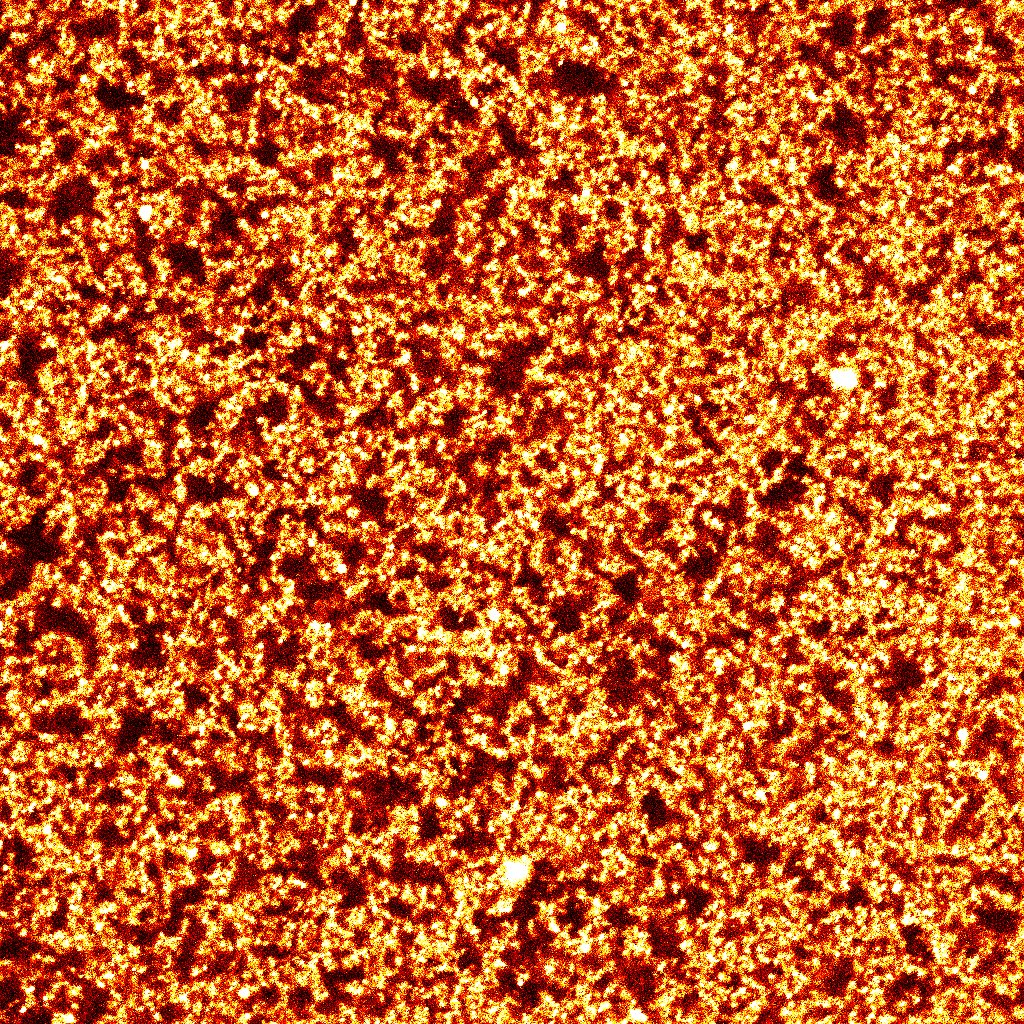
\includegraphics[width=0.45\textwidth]{XYslice_gly0.jpg}&
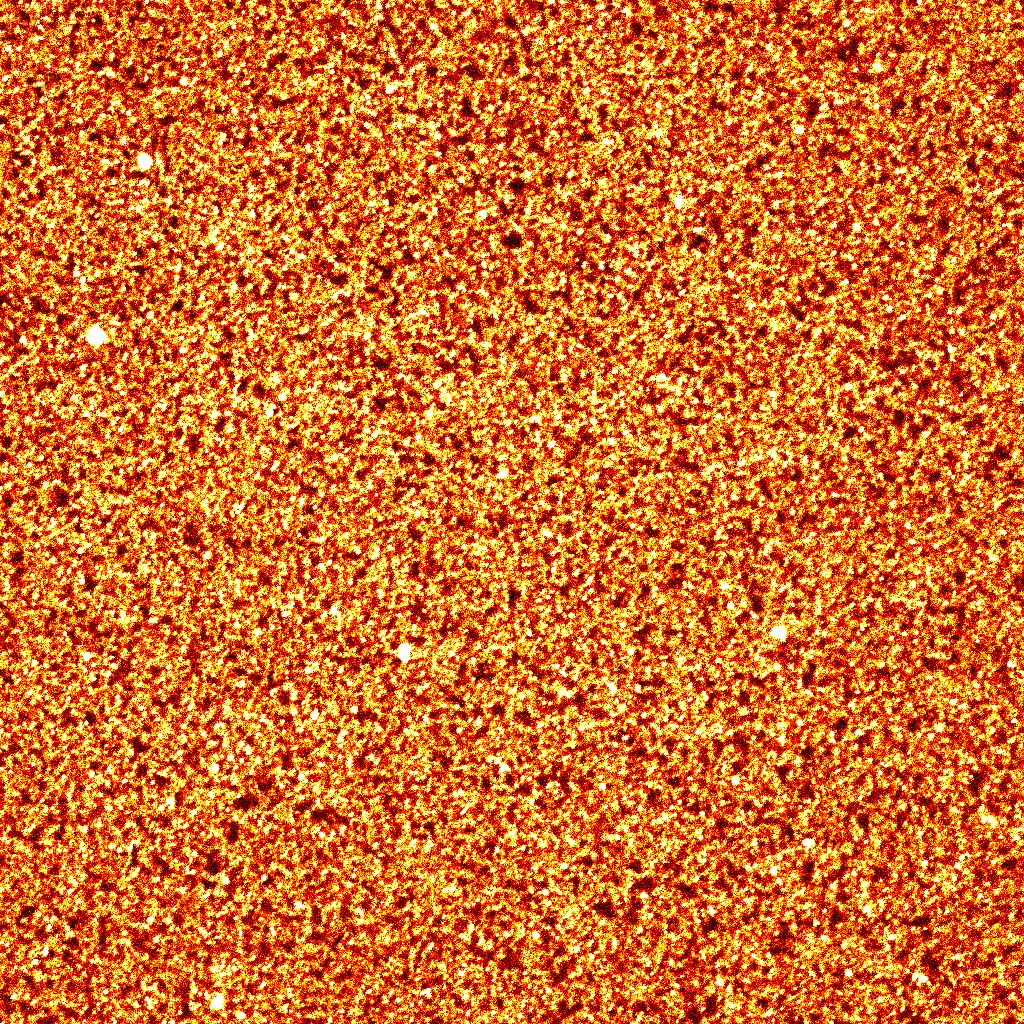
\includegraphics[width=0.45\textwidth]{XYslice_gly60.jpg}
\end{tabu}
\tikzsetnextfilename{scalebar_viscosty}
\tikz\draw[line width=0.2em] (0,0) -- ++(0.045\textwidth,0) node[midway, below] {\SI{10}{\micro\metre}};

May be explained by ``viscoelastic phase separation'' arguments
\end{frame}

\begin{frame}{Darcy vs Poiseuille}
\tikzsetnextfilename{Darcy_vs_Poiseuille}%
\begin{tikzpicture}
\pgfplotscreateplotcyclelist{accents}{%
	only marks,mark=*\\%
	only marks,mark=square*\\%
	black, no marks\\%
	black, no marks, dashed\\%
}

\begin{groupplot}[group style={
			group name=g, 
	group size=3 by 1,
	horizontal sep=1em,
	y descriptions at=edge left,
			},
	scale only axis,
	width=0.333\textwidth-1.66em,
	xmin=0, xmax=3,ymin=0,ymax=3,
	ylabel={$\lambda_\mathrm{exp}$ (\si{\milli\metre})},
	cycle list name=accents,
		colormap={accents}{color=(black) color=(yellow!25!red) color=(yellow!90!red)},
	point meta min=-1, point meta max=1,
	]
\nextgroupplot[xlabel={$\lambda$ Darcy (\si{\milli\metre})}]
\addplot+[scatter, error bars/.cd,x dir=both,y dir=both, x explicit,y explicit] table[x=D, x error=pmD, y=I, y error=pmI, scatter src={ln(\thisrow{ratio})/ln(10)}]{plis.txt};
\addplot+[scatter, error bars/.cd,x dir=both,y dir=both, x explicit,y explicit] table[x=Darcy, x error=pmD, y expr={\thisrow{Inter}/2}, y error expr={\thisrow{pmI}}, scatter src={ln(\thisrow{ratio})/ln(10)}]{plis_secondaires.txt};
\addplot[black] {0.63*x};



\nextgroupplot[xlabel={$\lambda$ Poiseuille (\si{\milli\metre})},
colorbar horizontal,
colorbar style={
	at={(0.5,0.95)}, anchor=north,
	width=0.5*\pgfkeysvalueof{/pgfplots/parent axis width},
	height=0.5em,
	xticklabel pos=lower,
	xlabel={$H/H^*$},
	xtick={-1, 0, 1},
	xticklabel=$10^{\pgfmathparse{\tick}\pgfmathprintnumber\pgfmathresult}$
},]
\addplot+[scatter, error bars/.cd,x dir=both,y dir=both, x explicit,y explicit] table[x=P, x error=pmP, y=I, y error=pmI, scatter src={ln(\thisrow{ratio})/ln(10)}]{plis.txt};
\addplot+[scatter, error bars/.cd,x dir=both,y dir=both, x explicit,y explicit] table[x=Poiseuille, x error=pmP, y expr={\thisrow{Inter}/2}, y error expr={\thisrow{pmI}}, scatter src={ln(\thisrow{ratio})/ln(10)}]{plis_secondaires.txt};
\addplot+[yellow!90!red] {0.69*x};
\addplot {0.52*x+0.33};

\nextgroupplot[xlabel={$\lambda_{D+P}$ (\si{\milli\metre})},]
\addplot+[scatter, error bars/.cd,x dir=both,y dir=both, x explicit,y explicit] table[x=M, x error=pmM, y=I, y error=pmI, scatter src={ln(\thisrow{ratio})/ln(10)}]{plis.txt};
\addplot+[scatter, error bars/.cd,x dir=both,y dir=both, x explicit,y explicit] table[x=Mixte, x error=pmM, y expr={\thisrow{Inter}/2}, y error expr={\thisrow{pmI}}, scatter src={ln(\thisrow{ratio})/ln(10)}]{plis_secondaires.txt};
\addplot+[yellow!25!red] {0.665*x};
\end{groupplot}

\end{tikzpicture}

\begin{itemize}
\item Poiseuille describes most of the data
\item Underestimates small wavelengths ($H\lesssim H^*$)
\item Fixed by a model taking both Darcy and Poiseuille into account
\end{itemize}

%\begin{center}
%Because desynchronisation
%
%\movie[externalviewer]{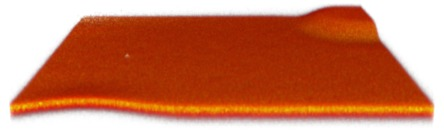
\includegraphics[width=0.5\textwidth]{volume_cloque_t116}}{volume_cloques_comp.avi}
%\end{center}

\end{frame}

\begin{frame}{Solvent is important in biogel mechanics}

\structure{Gel formation}
\begin{itemize}
	\item non adhesive boundary conditions $\Rightarrow$ synæresis
	\item gel properties depend on solvent viscosity
\end{itemize}

\bigskip
\structure{Non monotonic $p$H dependence}
\begin{itemize}
	\item spontaneous re-swelling $\Rightarrow$ biaxial compression
	\item lateral confinement $\Rightarrow$ cascade buckling, nested structures.
\end{itemize}

\bigskip
\structure{Gel poroelasticity}
\begin{itemize}
	\item porous flow resist bending
	\item Darcy may beat Poiseuille
	\item Asynchronous Poiseuille is preferred over Darcy
\end{itemize}


\end{frame}
